\documentclass{standalone}
\usepackage{graphicx}	
\usepackage{amssymb, amsmath}
\usepackage{color}

\usepackage{tikz}
\usetikzlibrary{intersections, backgrounds, math}
\usepackage{pgfmath}

\definecolor{light}{RGB}{220, 188, 188}
\definecolor{mid}{RGB}{185, 124, 124}
\definecolor{dark}{RGB}{143, 39, 39}
\definecolor{highlight}{RGB}{180, 31, 180}
\definecolor{gray10}{gray}{0.1}
\definecolor{gray20}{gray}{0.2}
\definecolor{gray30}{gray}{0.3}
\definecolor{gray40}{gray}{0.4}
\definecolor{gray60}{gray}{0.6}
\definecolor{gray70}{gray}{0.7}
\definecolor{gray80}{gray}{0.8}
\definecolor{gray90}{gray}{0.9}
\definecolor{gray95}{gray}{0.95}


\begin{document}

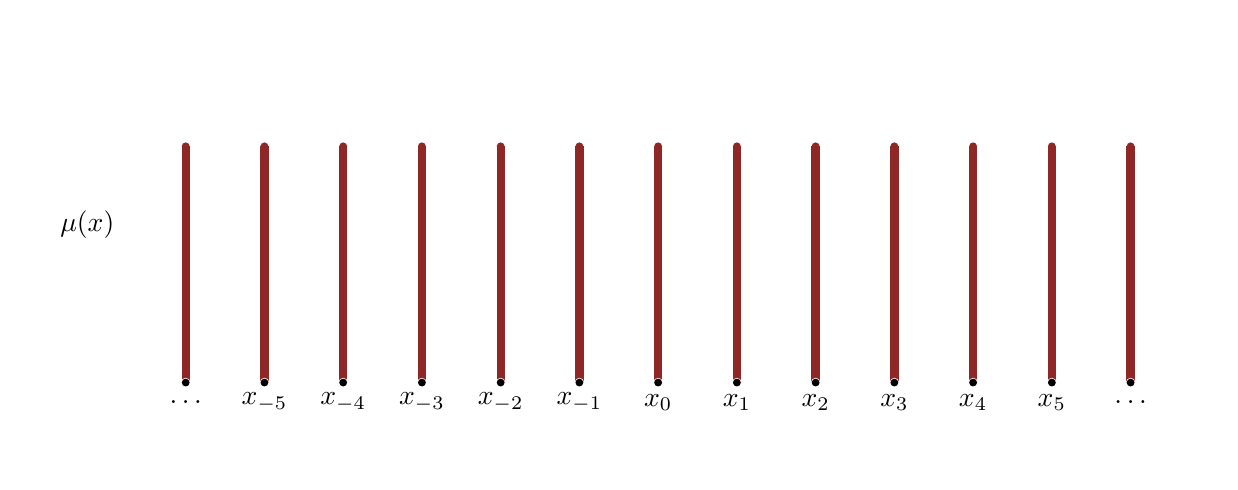
\begin{tikzpicture}[scale=1]
  \begin{scope}[shift={(0, 0)}]
    \draw[white] (-9, -3) rectangle (6, 2.5);
    
    \foreach [count=\n] \m in {0.2, 0.2, 0.2, 0.2, 0.2, 0.2, 0.2, 0.2, 0.2, 0.2, 0.2} {
      \pgfmathsetmacro{\x}{1.0 * ( (\n - 1) - 6)};
      \draw[dark, line width=3] (\x, -2) -- (\x, {(15 * \m - 2)});
      \fill[dark] (\x, {(15 * \m - 2)}) circle (0.05);
      \fill[white] (\x, -2) circle (0.06);
      \fill[black] (\x, -2) circle (0.05);
      
      \pgfmathtruncatemacro{\nn}{\n - 6};
      \node at (\x, -2.25) { $x_{\nn}$ };
    }
    
    \draw[dark, line width=3] (-7, -2) -- (-7, {(15 * 0.2 - 2)});
    \fill[dark] (-7, {(15 * 0.2 - 2)}) circle (0.05);
    \fill[white] (-7, -2) circle (0.06);
    \fill[black] (-7, -2) circle (0.05);
    \node at (-7, -2.25) { $\ldots$ };
 
    \draw[dark, line width=3] (5, -2) -- (5, {(15 * 0.2 - 2)});
    \fill[dark] (5, {(15 * 0.2 - 2)}) circle (0.05);   
    \fill[white] (5, -2) circle (0.06);
    \fill[black] (5, -2) circle (0.05);
    \node at (5, -2.25) { $\ldots$ };
 
    \node at (-8.25, 0) { $\mu(x)$ };
  \end{scope}
  
\end{tikzpicture}

\end{document}  